%------------------------------------------------
%	PACKAGES AND THEMES
%------------------------------------------------

% this is a 4:3 layout.
\documentclass{beamer}
% for 16:9 use this command:
% \documentclass[aspectratio=169]{beamer}

\mode<presentation> {
\usetheme{metropolis}
\setbeamertemplate{caption}[numbered]
\setbeamertemplate{navigation symbols}{} % hide navigation symbols
}

\usepackage{graphicx} % images
\usepackage{algorithm2e}
\usepackage{mathtools}
\DeclarePairedDelimiter{\ceil}{\lceil}{\rceil}
\usepackage{algpseudocode}
\usepackage{booktabs} % allows the use of \toprule, \midrule and \bottomrule in tables
\usepackage[ngerman]{babel}
\usepackage[utf8]{inputenc}
\usepackage[T1]{fontenc}
\usepackage{mathtools}
\usepackage{xcolor}
\usepackage{listings} % code
\usepackage{pgf,tikz} % drawing
\usepackage{pifont} % new symbols
\usepackage{hyperref} % pretty links
% \usepackage{algorithmicx}
% \usepackage{algpseudocode}
% \usepackage[linesnumbered,ruled]{algorithm2e}

\usepackage{lmodern}
\usepackage{subcaption}
\usepackage{textcomp}
% \usepackage{array}
% \usepackage{longtable}
% \usepackage{verbatim}
%\usepackage{tabularx}
\captionsetup[figure]{font=footnotesize}

\usepackage{amsmath}
\usepackage{amssymb}
\usepackage{amsthm}
% \usepackage{comment}
% \usepackage{enumitem}
% \usepackage[binary-units=true]{siunitx}
% \usepackage{thmtools}
\usepackage{csquotes}
\usepackage{tikz}
\usepackage{float}
\usetikzlibrary{automata,positioning}

% color settings for links
\hypersetup{
    colorlinks=true,
    urlcolor=blue,
    linkcolor=black,
    citecolor=green!50!black
}

\definecolor{mygreen}{RGB}{1,135,1}

\newcommand{\cmark}{\ding{51}}  % checkmark
\newcommand{\xmark}{\ding{55}}  % xmark
\newcommand\scalemath[2]{\scalebox{#1}{\mbox{\ensuremath{\displaystyle #2}}}}

% \useoutertheme{miniframes} % navigation design
\useinnertheme{circles} % use non shiny circles (itemize, etc.)

% Main slide colors
% dunkel, hell, mittel
% \definecolor{pale}{RGB}{232, 236, 237}
% \definecolor{prim}{RGB}{53, 109, 120}
% \definecolor{sec}{RGB}{104, 170, 183}
% \definecolor{tert}{RGB}{109, 155, 168}
% \definecolor{quat}{RGB}{9, 59, 68}

\definecolor{pale}{RGB}{232, 236, 237}
% \definecolor{prim}{RGB}{153, 194, 173}
% good: \definecolor{prim}{RGB}{27, 33, 42}
\definecolor{prim}{RGB}{32, 43, 50}
\definecolor{sec}{RGB}{217, 232, 224}
\definecolor{tert}{RGB}{0, 82, 41}
% save
\definecolor{quat}{RGB}{0, 82, 41}

\setbeamercolor{palette primary}{bg=prim,fg=pale}
\setbeamercolor{palette secondary}{bg=sec,fg=pale}
\setbeamercolor{palette tertiary}{bg=tert,fg=pale}
\setbeamercolor{palette quaternary}{bg=quat,fg=pale}
\setbeamercolor{structure}{fg=prim} % itemize, enumerate, etc
\setbeamercolor{section in toc}{fg=prim} % TOC sections

% Block colors
\definecolor{example_color}{RGB}{93, 137, 98}
\definecolor{alert_color}{RGB}{175, 79, 72}

\setbeamercolor{normal text}{fg=prim!20!black,bg=pale!25!white}
\setbeamercolor{alerted text}{fg=alert_color!25!black}
\setbeamercolor{example text}{fg=example_color!25!black}

\setbeamercolor{block title example}{fg=white,bg=example_color}
\setbeamercolor{block body example}{fg=black,bg=example_color!10!white}
\setbeamercolor{block title alerted}{fg=white,bg=alert_color}
\setbeamercolor{block body alerted}{fg=black,bg=alert_color!10!white}

% Override palette coloring
\setbeamercolor{subsection in head/foot}{bg=quat,fg=pale}

\setbeamertemplate{frametitle}{%
    \nointerlineskip%

    \begin{beamercolorbox}[wd=\paperwidth,ht=2.5ex,dp=1ex]{frametitle}
        \hspace*{1ex}\insertframetitle%
        \ifx\insertframesubtitle@empty\else%
        {~\tiny\textcolor{quat!35!black}{\insertframesubtitle}}%
        \fi%
    \end{beamercolorbox}%
}

% math-command for bigger norm
\newcommand\norm[1]{\left\lVert#1\right\rVert}

% use this to include other files
% in this case style definitions for code
% alternative: \include{dateiname}
\lstdefinestyle{latex}{
    language=[LaTeX]TeX,
    inputencoding=utf8,
    basicstyle=\ttfamily,
    keywordstyle=\color{blue!60!black}, % use 60 percent blue and 40 black
    commentstyle=\color{cyan!60!black},
    tabsize=2,
    emph={document,itemize,enumerate,center,tabular,table,
    figure,wrapfigure,minipage,columns,align,bmatrix,
    lstlisting,beamer,frame,tikzpicture},
    emphstyle=\color{magenta!60!black},
    morekeywords={lstset,includegraphics,theenumi,labelitemi,column,color,url,href}
}

\lstdefinestyle{inline_latex}{
    language=[LaTeX]TeX,
    inputencoding=utf8,
    basicstyle=\ttfamily,
    resetmargins= true,
    belowcaptionskip=0pt,
    aboveskip=0pt,
    belowskip=0pt,
    keywordstyle=\color{blue!60!black},
    commentstyle=\color{cyan!60!black},
    emph={document,itemize,enumerate,center,tabular,table,
    figure,wrapfigure,minipage,columns,align,bmatrix,
    lstlisting,beamer,frame,tikzpicture,Parameter},
    emphstyle=\color{magenta!60!black},
    morekeywords={lstset,includegraphics,theenumi,labelitemi,column,color,url,href,Befehlsname}
}

\lstdefinestyle{cpp}{
    language=C++,
    basicstyle=\ttfamily,
    keywordstyle=\color{blue!90!black},
    stringstyle=\color{magenta!60!black},
    commentstyle=\color{green!35!black},
    morecomment=[l][\color{gray!60!black}]{\#},
    tabsize=2
}

\lstdefinestyle{empty}{
    basicstyle=\rmfamily,
    keywordstyle=\bfseries,
    commentstyle=\color{black}\itshape
}

\lstset{style=latex}

%------------------------------------------------
%	TITLE PAGE
%------------------------------------------------

\selectlanguage{ngerman}
\title[]{Heuristische Lösungsverfahren für Stacking-Probleme mit Transportkosten}

\author{Tim Bohne}
\institute[]
{
\textit{AG Kombinatorische Optimierung}
\medskip
}
\date{\today}

% make slide at the beginnig of each section
\AtBeginSection[]{
{\setbeamercolor{background canvas}{bg=white}}}

% where images are locatied
\graphicspath{{./images/}}

\begin{document}

\begin{frame}[plain] % plain slides dont have navigation bars etc.
\titlepage % Print the title page as the first slide
\end{frame}

\begin{frame}
\frametitle{Übersicht} % table of contents slide
\tableofcontents
\end{frame}

%------------------------------------------------
\section{Stacking-Probleme}
%------------------------------------------------
% \subsection*{}

\begin{frame}
\frametitle{Stacking-Probleme}
\begin{itemize}
\item Im Umfeld von Lagerhallen und Container-Terminals
\item Eintreffende Items müssen Stacks zugeordnet werden, sodass bestimmte Nebenbedingungen respektiert werden
\item Storage Area ist in fixierten Stacks organisiert, die eine limitierte gemeinsame Stack Kapazität besitzen
% \item Item-Zugriff erfolgt nach dem \textquote{Last-In–First-Out}-Prinzip
\item Es wird nur der Loading-Prozess betrachtet
\end{itemize}
\begin{figure}
\centering
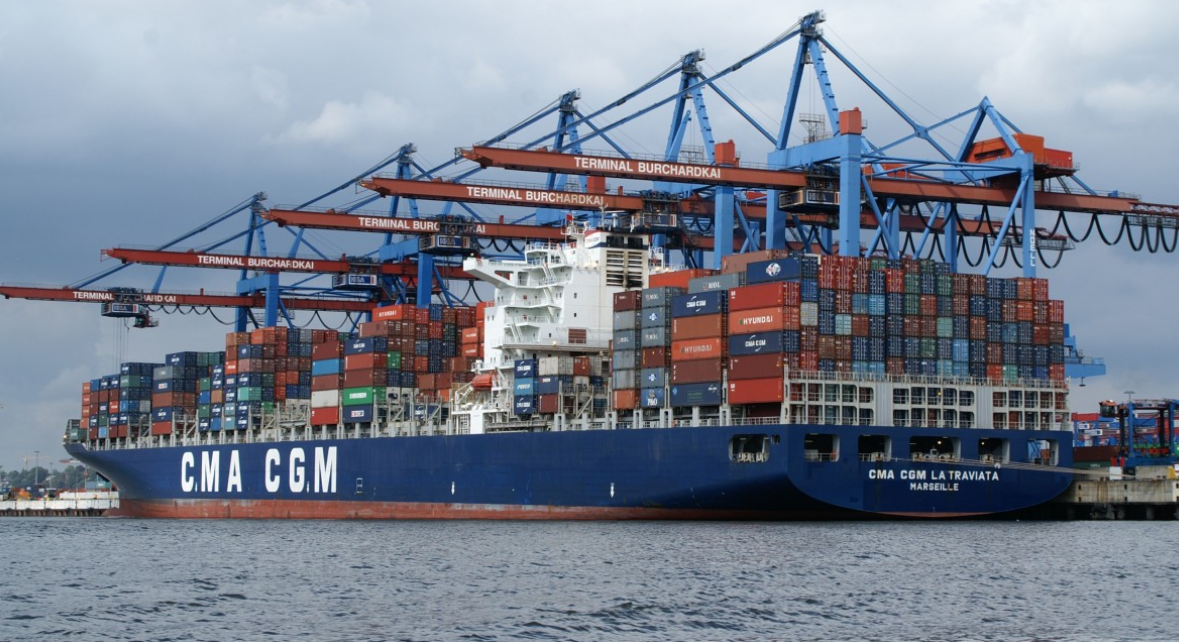
\includegraphics[width=0.8\textwidth]{images/t5.png}
\end{figure}
\end{frame}

\begin{frame}
\frametitle{Literatur Überblick}

\begin{itemize}
  \item \textbf{Kim et al. (2000)}: Deriving decision rules to locate export containers in container yards
  \item \textbf{Kang et al. (2006)}: Deriving stacking strategies for export containers with uncertain weight information
  \item \textbf{Delgado et al. (2012)}: A constraint programming model for fast optimal stowage of container vessel bays
  \item \textbf{Jaehn (2013)}: Positioning of loading units in a transshipment yard storage area
  \item \textbf{Bruns et al. (2015)}: Complexity results for storage loading problems with stacking constraints
  \item \textbf{Le et al. (2016)}: MIP-based approaches for robust storage loading problems with stacking constraints
  % \item \textbf{Caserta et. al. (2012)}: A mathematical formulation and complexity considerations for the blocks relocation problem.
\end{itemize}

\end{frame}

\begin{frame}
\frametitle{Storage Area}
Aufbau der Storage Area bestehend aus $\boldsymbol{m}$ fixierten Stacks, die jeweils $\boldsymbol{b}$ Level enthalten:\newline

\begin{figure}[H]
\centering
\resizebox{0.6\textwidth}{!}{
\begin{tabular}{|c|c|c|c|c|c|}
\cline{1-5}
$\boldsymbol{S_1}$ & $\boldsymbol{S_2}$ & $\boldsymbol{S_3}$ & ... & $\boldsymbol{S_m}$\\ \cline{1-5}
\end{tabular}}
\caption*{\textsc{von oben betrachtet}}
\end{figure}

\begin{figure}[H]
\centering
\resizebox{0.6\textwidth}{!}{
\begin{tabular}{c|c|c|c|c|c|}
\cline{2-6}
$\boldsymbol{L_b}$ & $pos_{1, b}$ & $pos_{2, b}$ & $pos_{3, b}$ & ... & $pos_{m, b}$ \\ \cline{2-6}
... & ... & ... & ... & ... & ...\\ \cline{2-6}
$\boldsymbol{L_2}$ & $pos_{1, 2}$ & $pos_{2, 2}$ & $pos_{3, 2}$ & ... & $pos_{m, 2}$\\ \cline{2-6}
$\boldsymbol{L_1}$ & $pos_{1, 1}$ & $pos_{2, 1}$ & $pos_{3, 1}$ & ... & $pos_{m, 1}$\\ \cline{2-6}
\multicolumn{1}{c}{} & \multicolumn{1}{c}{$\boldsymbol{S_1}$} & \multicolumn{1}{c}{$\boldsymbol{S_2}$}
& \multicolumn{1}{c}{$\boldsymbol{S_3}$} & \multicolumn{1}{c}{...} & \multicolumn{1}{c}{$\boldsymbol{S_m}$} \\
\end{tabular}}
\caption*{\textsc{von der Seite betrachtet}}
\end{figure}
\end{frame}

\begin{frame}
\frametitle{Stacking-Probleme}
\begin{figure}[H]
\centering
\resizebox{0.7\textwidth}{!}{
\begin{tabular}{ | l | l |}
    \hline
    \textbf{Parameter} & \textbf{Semantik} \\ \hline
    $n$ & Anzahl der Items \\ \hline
    $m$ & Anzahl der Stacks \\ \hline
    $b$ & Stack Kapazität \\ \hline
    $I$ & Menge der Items $ I := \{1, 2, ..., n\}$ \\ \hline
\end{tabular}}
\end{figure}
\centering
I.d.R. gilt $\boldsymbol{m} < \boldsymbol{n}$, außerdem muss $\boldsymbol{n} \leq \boldsymbol{bm}$ gelten.
\end{frame}

\begin{frame}
\frametitle{Stacking-Probleme}

\textbf{Formulierung des Problems}\newline

Items: $\boldsymbol{I} = \{1, ..., n\}$\newline
Stacks: $\boldsymbol{Q} = \{1, ..., m\}$\newline
Stack Kapazität: $\boldsymbol{b}$\newline
Stacking Constraints: $\boldsymbol{s_{ij}}$\newline
Placement Constraints: $\boldsymbol{t_{iq}}$\newline

Das Ziel ist, jedes Item $\boldsymbol{i} \in \boldsymbol{I}$ genau einem Stack $\boldsymbol{q} \in \boldsymbol{Q}$ zuzuweisen,
wobei die Stacking Constraints $\boldsymbol{s_{ij}}$, die Placement Constraints $\boldsymbol{t_{iq}}$ und die Stack Kapazität $\boldsymbol{b}$ respektiert werden und ggf. eine Zielfunktion optimiert wird.
\end{frame}

%------------------------------------------------
\section{Nebenbedingungen}
%------------------------------------------------
% \subsection*{}

\begin{frame}
\frametitle{Stacking Constraints}
\begin{itemize}
    \item Schwerere Items dürfen nicht auf leichteren platziert werden
    \item Größere Items dürfen nicht auf kleineren platziert werden
    \item Items bestimmter Materialien / Zielorte dürfen nicht aufeinander gestapelt werden\newline
\end{itemize}
Sämtliche Stacking Constraints werden in einer Binärmatrix $\boldsymbol{S} = (\boldsymbol{s_{ij}})_{n \times n}$ kodiert, wobei:
\[
    \boldsymbol{s_{ij}} =
\begin{cases}
    1, & \text{wenn $\boldsymbol{i}$ direkt auf $\boldsymbol{j}$ gestapelt werden darf }\\
    0, & \text{sonst}
\end{cases}
\]
\end{frame}

\begin{frame}
\frametitle{Stacking Constraints}
Diese Matrix lässt sich als gerichteter Graph mit $\boldsymbol{n}$ Knoten $\boldsymbol{i} \in \boldsymbol{I}$ \newline und Kanten $\boldsymbol{i} \rightarrow \boldsymbol{j}$ für alle $\boldsymbol{s_{ij}} = 1$ repräsentieren.\newline

\begin{figure}[H]
  \begin{subfigure}[b]{0.45\textwidth}
  \centering
    $\boldsymbol{S} =$
    $\left(
    \begin{array}{rrrr}
    0 & 1 & 1 & 0 \\
    1 & 0 & 1 & 0 \\
    1 & 0 & 0 & 0 \\
    1 & 1 & 1 & 0 \\
    \end{array} \right) $
    \caption*{\textsc{Constraint Matrix}}
  \end{subfigure}
  \hfill
  \begin{subfigure}[b]{0.45\textwidth}
  \centering
    \begin{tikzpicture}[->, scale=0.50, transform shape, node distance=2.5cm]
    \node[state] (A) {1};
    \node[state] (B) [right of=A] {2};
    \node[state] (C) [below of=A] {3};
    \node[state] (D) [right of=C] {4};

    \path (A) edge node {} (B)
          (A) edge node {} (C)
          (B) edge [bend right] node {} (A)
          (B) edge [bend left=10] node {} (C)
          (C) edge [bend left] node {} (A)
          (D) edge [bend left=10] node {} (A)
          (D) edge node {} (B)
          (D) edge node {} (C);
  \end{tikzpicture}
    \caption*{\textsc{Resultierender Graph}}
  \end{subfigure}
  \newline
\end{figure}
\end{frame}

\begin{frame}
\frametitle{Stacking-Constraint-Generierung}
\textbf{Variante 1:}
\begin{itemize}
  \item $\boldsymbol{S}$ anhand definierter Wahrscheinlichkeit mit 1/0 Werten füllen
  \item 1-Einträge, die aus Transitivität folgen, ergänzen
\end{itemize}
\textbf{Variante 2:}
\begin{itemize}
  \item Für alle $\boldsymbol{n}$ Items zufällige Länge und Breite generieren
  \item Item $\boldsymbol{i}$ kann auf Item $\boldsymbol{j}$ platziert werden, wenn für dessen Länge $\boldsymbol{l_i}$ und Breite
  $\boldsymbol{w_i}$ gilt $\boldsymbol{l_i} \leq \boldsymbol{l_j}$ und $\boldsymbol{w_i} \leq \boldsymbol{w_j}$
  \item Items $\boldsymbol{i}, \boldsymbol{j}$ sind in beide Richtungen stackbar, wenn $\boldsymbol{l_i} =
  \boldsymbol{l_j}$ und $\boldsymbol{w_i} = \boldsymbol{w_j}$
\end{itemize}
\end{frame}

\begin{frame}
\frametitle{Transportkosten}

\begin{itemize}
  \item Kranbetriebskosten, Wartezeiten, Arbeitszeiten, ...
  \item Jeder Stack $\boldsymbol{q}$ hat eine fixierte Position $\boldsymbol{F_q}$ in der Storage Area
  \item Jedes Item $\boldsymbol{i}$ hat eine geg. Originalposition $\boldsymbol{O_i}$ auf dem Fz.
\end{itemize}

Die Kosten werden in einer Matrix $\boldsymbol{C} = (\boldsymbol{c_{iq}})_{n \times m}$ kodiert.\newline
$\boldsymbol{c_{iq}} \coloneqq d_{man}(\boldsymbol{O_i}, \boldsymbol{F_q})$

\begin{figure}[H]
\centering
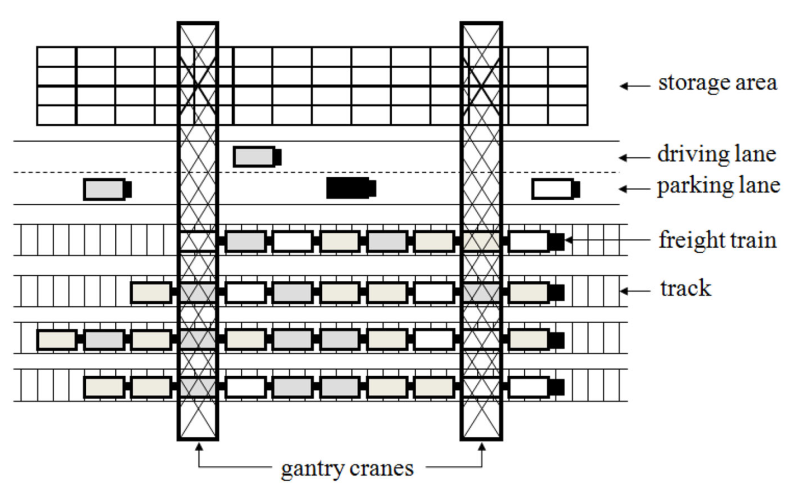
\includegraphics[width=0.75\textwidth]{images/costs.png}\newline
\end{figure}

\end{frame}

\begin{frame}
\frametitle{Placement Constraints}
\begin{itemize}
    \item Länge / Gewicht der Items und Eigenschaften der Stacks
    \item Spezielle Anforderungen der Items (Kühlcontainer, ...)
    \item Tendenziell mehr erlaubt als verboten (rand(0, 1) zu restriktiv)
    \item Über sehr hohe Kostenwerte umgesetzt\newline
\end{itemize}
In Binärmatrix $\boldsymbol{T} = (\boldsymbol{t_{iq}})_{n \times m}$ kodiert, wobei:
$
    \boldsymbol{t_{iq}} =
\begin{cases}
    1, & \text{wenn Item $\boldsymbol{i}$ in Stack $\boldsymbol{q}$ platziert werden darf }\\
    0, & \text{sonst}
\end{cases}
$
\\[20pt]
Für die Transportkosten-Matrix $\boldsymbol{C} = (\boldsymbol{c_{iq}})_{n \times m}$ gilt:
$
    \boldsymbol{c_{iq}} =
\begin{cases}
    d_{man}(\boldsymbol{O_i}, \boldsymbol{F_q}), & \text{wenn $\boldsymbol{t_{iq}} = 1$}\\
    \infty, & \text{sonst}
\end{cases}
$
\end{frame}

%------------------------------------------------
\section{Settings / Testdaten}
%------------------------------------------------

\begin{frame}
\frametitle{Problem Settings}

\textbf{Stack-Kapazitäten}: $\boldsymbol{b} = 2, 3, (4)$
\begin{itemize}
  \item Zulässigkeitsproblem $\boldsymbol{b=2}$ mit $\boldsymbol{s_{ij}}$ und $\boldsymbol{t_{iq}}$ NP-schwer
  \item Zulässigkeitsproblem $\boldsymbol{b=3}$ mit $\boldsymbol{s_{ij}}$ NP-schwer
\end{itemize}

\textbf{Instanzgrößen}:
\begin{itemize}
  \item klein (\textbf{s}) ($\leq 100$ Items)
  \item mittel (\textbf{m}) ($\approx 300$ Items)
  \item groß (\textbf{l}) ($\approx 500$ Items)\newline
\end{itemize}

\textbf{Ziel}: Sämtliche Items sollen möglichst günstig eingelagert werden.\newline
\textbf{Zielfunktion}: Minimierung der Transportkosten\newline

\textbf{Zulässigkeit und geringe Laufzeit haben Priorität.}\newline
\end{frame}

\begin{frame}
\frametitle{Zulässigkeit}
\textbf{Kriterien für die Zulässigkeit einer Lösung}:
\begin{itemize}
  \item Sämtliche Items eingelagert
  \item Stacking Constraints respektiert
  \item Placement Constraints respektiert
\end{itemize}

Die Placement Constraints gelten als verletzt, wenn eine Lösung eine Item-Zuweisung der Kosten $\infty$ enthält.
\end{frame}

\begin{frame}
\frametitle{Testdaten-Generierung}

\begin{itemize}
  \item Anzahl der Instanzen: \textcolor{red}{$\boldsymbol{20}$}\newline
  \item Anzahl der Items: $\boldsymbol{n}$
  \item Stack Kapazität: $\boldsymbol{b}$
  \item Anzahl der Stacks: $\boldsymbol{m}$ = $\ceil{\boldsymbol{n} / \boldsymbol{b}}$ + $\textcolor{red}{\boldsymbol{20 \%}}$\newline
  \item Stacking Constraints: \textcolor{red}{\textbf{Variante 2}}
  \item Placement Constraints: $\textcolor{red}{\boldsymbol{70 \%}}$ erlaubt
  \item Kosten: \textcolor{red}{\textbf{Manhattan-Metrik}}
  \begin{itemize}
    \item Item- und Stackpositionen ($x, y$)
    \item Item- und Stack-Längen, Item- und Stack-Breiten
    \item Distanz zwischen Storage Area und Fahrzeug
  \end{itemize}
\end{itemize}
\end{frame}

%------------------------------------------------
\section{Heuristiken / Vergleich}
%------------------------------------------------

\begin{frame}
\frametitle{MIP Formulierungen}
\centering
\textbf{Bin-Packing-Formulierung}
\scalebox{0.7}{\parbox{\linewidth}{%
\begin{gather}
\boldsymbol{min} \quad \sum_{i \in I} \sum_{q \in Q} c_{iq} x_{iq} \\
\thinspace\thinspace \boldsymbol{s.t.} \thinspace \quad \sum_{q \in Q} x_{iq} = 1 \thinspace\thinspace\quad\quad\quad\quad\quad \forall i \in I \quad\quad\quad\quad\thinspace \\
\quad \sum_{i \in I} x_{iq} \leq b \quad\quad\quad\quad\quad\quad\quad \forall q \in Q \\
\thinspace\thinspace\quad\quad x_{iq} + x_{jq} \leq 1 \quad\quad\thinspace\thinspace\quad\quad\quad\quad \forall \{i, j\} \notin A \\
\thinspace\thinspace\quad\quad\quad x_{iq} \in \{0, 1\} \thinspace\thinspace\thinspace\thinspace\thinspace\thinspace\quad\quad\quad\quad\quad\quad \forall i \in I, q \in Q \thinspace
\end{gather}}}
\centering
\textbf{3-Index-Formulierung}
\scalebox{0.7}{\parbox{\linewidth}{%
\begin{gather}
\boldsymbol{min} \quad \sum_{i \in I} \sum_{q \in Q} \sum_{l \in L} c_{iq} x_{iql} \\
\boldsymbol{s.t.} \quad \sum_{q \in Q} \sum_{l \in L} x_{iql} = 1 \quad\thinspace\thinspace\quad\quad\quad\quad \forall i \in I \thinspace\thinspace\quad\quad\quad\quad\quad\quad\quad\quad\thinspace\thinspace \\
\sum_{i \in I} x_{iql} \leq 1 \thinspace\quad\quad\quad\quad\quad\quad\quad \forall q \in Q, l \in L \thinspace\thinspace\thinspace\thinspace\quad\quad\quad\thinspace \\
\sum_{j \in I | i \rightarrow j} x_{jq(l-1)} - x_{iql} \geq 0 \thinspace\quad\quad \forall i \in I, q \in Q, l \in L \textbackslash \{1\} \\
\quad\quad x_{iql} \in \{0, 1\} \quad\quad\quad\quad\quad\quad\quad \forall i \in I, q \in Q, l \in L \quad\thinspace\thinspace\thinspace\thinspace\thinspace
\end{gather}}}


% 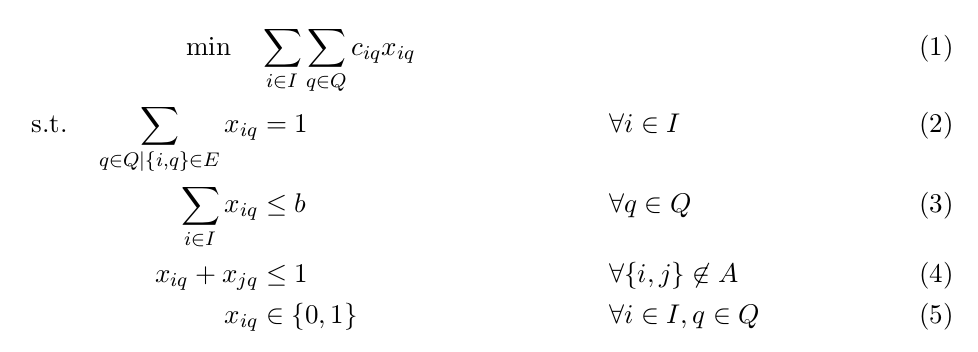
\includegraphics[width=0.75\textwidth]{images/BinP.png}\newline
% 3-Index Formulierung\newline
% 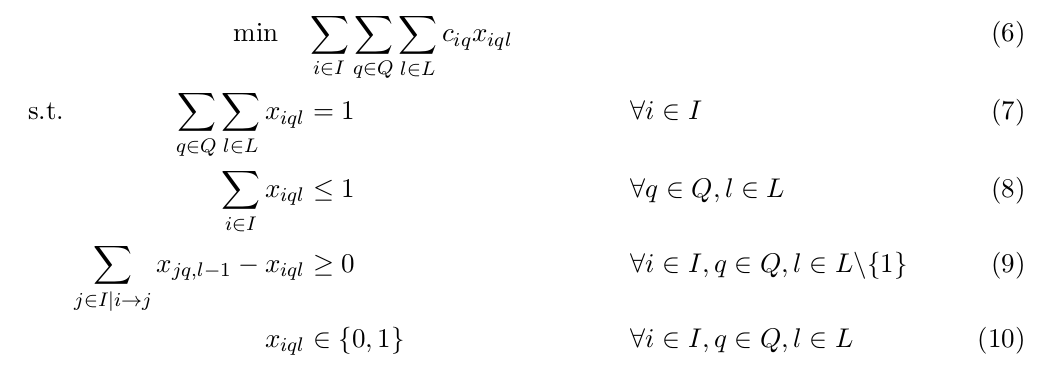
\includegraphics[width=0.75\textwidth]{images/3Idx.png}
\end{frame}

% \begin{frame}
% \frametitle{MIP Formulierungen}
% \textbf{Kleine Instanzen} ($b = 2$, $30$s Zeitlimit, Schwierigkeit: 25\%)
% \begin{figure}[H]
% \centering
% \resizebox{0.5\textwidth}{!}{
% \begin{tabular}{ | l | l | l |}
%     \hline
%      & \textbf{BinP} & \textbf{3Idx} \\ \hline
%     \textbf{\textquote{Instance Coverage}} & 100\% & 100\% \\ \hline
%     \textbf{Kosten} & \O $\thinspace 102$ & \O  $\thinspace 102$ \\ \hline
%     \textbf{Laufzeit} & \O $\thinspace \textcolor{red}{3.6s}$ & \O  $\thinspace \textcolor{mygreen}{2.3s}$ \\ \hline
% \end{tabular}}
% \caption*{Kein Bedarf für Laufzeitverbesserung durch Heuristik!}
% \end{figure}

% \textbf{Mittlere Instanzen} ($b = 2$, $180$s Zeitlimit, Schwierigkeit: 25\%)

% \begin{figure}[H]
% \centering
% \resizebox{0.5\textwidth}{!}{
% \begin{tabular}{ | l | l | l |}
%     \hline
%      & \textbf{BinP} & \textbf{3Idx} \\ \hline
%     \textbf{\textquote{Instance Coverage}} & 100\% & 100\% \\ \hline
%     \textbf{Kosten} & \O $\thinspace \textcolor{red}{466}$ & \O  $\thinspace \textcolor{mygreen}{300}$ \\ \hline
%     \textbf{Laufzeit} & \O $\thinspace \textcolor{red}{154s}$ & \O  $\thinspace \textcolor{mygreen}{40s}$ \\ \hline
% \end{tabular}}
% \end{figure}

% \end{frame}

% \begin{frame}
% \frametitle{MIP Formulierungen}

% \textbf{Große Instanzen} ($b = 2$, $300$s Zeitlimit, Schwierigkeit: 25\%)

% \begin{figure}[H]
% \centering
% \resizebox{0.5\textwidth}{!}{
% \begin{tabular}{ | l | l | l |}
%     \hline
%      & \textbf{BinP} & \textbf{3Idx} \\ \hline
%     \textbf{\textquote{Instance Coverage}} & \textcolor{red}{0\%} & \textcolor{mygreen}{70\%} \\ \hline
%     \textbf{Kosten} & \textcolor{red}{$-$} & \O  $\thinspace \textcolor{mygreen}{619}$  \\ \hline
%     \textbf{Laufzeit} & \textcolor{red}{$-$} & \O  $\thinspace \textcolor{mygreen}{191s}$  \\ \hline
% \end{tabular}}
% \end{figure}

% \textbf{Kleine Instanzen} ($b = 3$, $30$s Zeitlimit, Schwierigkeit: 25\%)
% \begin{figure}[H]
% \centering
% \resizebox{0.5\textwidth}{!}{
% \begin{tabular}{ | l | l | l |}
%     \hline
%      & \textbf{BinP} & \textbf{3Idx} \\ \hline
%     \textbf{\textquote{Instance Coverage}} & \textcolor{mygreen}{$75$\%} & \textcolor{red}{$45$\%} \\ \hline
%     \textbf{Kosten} & \O $\thinspace \textcolor{mygreen}{133}$ & \O  $\thinspace \textcolor{red}{150}$ \\ \hline
%     \textbf{Laufzeit} & \O $\thinspace \textcolor{mygreen}{19s}$ & \O  $\thinspace \textcolor{red}{26s}$ \\ \hline
% \end{tabular}}
% \end{figure}

% \end{frame}

% \begin{frame}
% \frametitle{MIP Formulierungen}

% \textbf{Mittlere Instanzen} ($b = 3$, $180$s Zeitlimit, Schwierigkeit: 25\%)

% \begin{figure}[H]
% \centering
% \resizebox{0.5\textwidth}{!}{
% \begin{tabular}{ | l | l | l |}
%     \hline
%      & \textbf{BinP} & \textbf{3Idx} \\ \hline
%     \textbf{\textquote{Instance Coverage}} & \textcolor{mygreen}{60\%} & \textcolor{red}{0\%} \\ \hline
%     \textbf{Kosten} & \O $\thinspace \textcolor{mygreen}{875}$ & $\textcolor{red}{-}$ \\ \hline
%     \textbf{Laufzeit} & \O $\thinspace \textcolor{mygreen}{180s}$ & $\textcolor{red}{-}$ \\ \hline
% \end{tabular}}
% \end{figure}

% \textbf{Große Instanzen} ($b = 3$, $300$s Zeitlimit, Schwierigkeit: 25\%)

% \begin{figure}[H]
% \centering
% \resizebox{0.5\textwidth}{!}{
% \begin{tabular}{ | l | l | l |}
%     \hline
%      & \textbf{BinP} & \textbf{3Idx} \\ \hline
%     \textbf{\textquote{Instance Coverage}} & \textcolor{mygreen}{25\%} & \textcolor{red}{0\%} \\ \hline
%     \textbf{Kosten} & \O $\thinspace \textcolor{mygreen}{2167}$ & $\textcolor{red}{-}$ \\ \hline
%     \textbf{Laufzeit} & \O $\thinspace \textcolor{mygreen}{300s}$ & $\textcolor{red}{-}$ \\ \hline
% \end{tabular}}
% \end{figure}

% \end{frame}

\begin{frame}
\frametitle{Exkurs: Maximum-Cardinality-Matching (\textsc{MCM})}
Ungerichteter Graph $\boldsymbol{G} = (\boldsymbol{V}, \boldsymbol{E})$\newline

Eine Menge $\boldsymbol{M} \subseteq \boldsymbol{E}$ heißt Matching, wenn keine zwei Kanten aus $\boldsymbol{M}$ einen Knoten gemeinsam haben.
\newline

Falls $\boldsymbol{M}$ eine maximale Kardinalität unter allen Matchings von $\boldsymbol{G}$ hat, wird dies als \textsc{MCM} bezeichnet.
\begin{figure}[H]
  \begin{subfigure}[b]{0.4\textwidth}
  \centering
    \begin{tikzpicture}[scale=0.45, transform shape, node distance=2cm]
    \node[state] (A) {};
    \node[state] (B) [above right of=A] {};
    \node[state] (C) [below left of=A] {};
    \node[state] (D) [below right of=C] {};
    \node[state] (F) [below right of=B] {};
    \node[state] (E) [below of=F] {};

    \path (A) edge [mygreen] node {} (B)
          (A) edge node {} (C)
          (A) edge node {} (D)
          (A) edge node {} (E)
          (A) edge node {} (F)
          (C) edge [mygreen] node {} (D);
  \end{tikzpicture}
  \caption*{\textsc{$|\textsc{MCM}| = 2$}}
  \end{subfigure}
  \hfill
  \begin{subfigure}[b]{0.4\textwidth}
  \centering
    \begin{tikzpicture}[scale=0.45, transform shape, node distance=2cm]
    \node[state] (A) {};
    \node[state] (B) [right of=A] {};
    \node[state] (C) [right of=B] {};
    \node[state] (D) [below left of=A] {};
    \node[state] (E) [below right of=D] {};
    \node[state] (F) [right of=E] {};

    \path (A) edge node {} (B)
          (B) edge [mygreen] node {} (C)
          (B) edge node {} (F)
          (A) edge node {} (E)
          (E) edge [mygreen] node {} (F)
          (A) edge [mygreen] node {} (D)
          (D) edge node {} (E);
  \end{tikzpicture}
    \caption*{\textsc{$|\textsc{MCM}| = 3$}}
  \end{subfigure}
\end{figure}
\end{frame}

\begin{frame}
\frametitle{Exkurs: Minimum-Weight-Perfect-Matching (\textsc{MWPM})}
\begin{itemize}
  \item Matching, welches sämtliche Knoten matcht
  \item Jeder Knoten ist inzident zu genau einer Kante des Matchings
  \item Günstigstes Perfect Matching basierend auf den Kantenkosten
\end{itemize}
\begin{figure}[H]
\centering
\begin{tikzpicture}[-, scale=0.5, transform shape, node distance=3cm]
    \node[state] (A) {};
    \node[state] (B) [above right of=A] {};
    \node[state] (C) [below right of=A] {};
    \node[state] (D) [right of=B] {};
    \node[state] (E) [right of=D] {};
    \node[state] (F) [right of=C] {};

    \path (A) edge [mygreen] node {} (B)
          (A) edge node {} (C)
          (B) edge node {} (D)
          (B) edge node {} (C)
          (D) edge [mygreen] node {} (E)
          (D) edge node {} (F)
          (C) edge [mygreen] node {} (F);
\end{tikzpicture}
\end{figure}
\end{frame}

\begin{frame}
\frametitle{Konstruktive Heuristik ($b = 2$)}

\begin{itemize}
  \item Stacking-Constraint-Graph generieren
  \item \textsc{\textbf{MCM}} berechnen, Kanten als Item-Paare interpretieren
  \item Bipartiten Graph generieren:
  \begin{enumerate}
    \item Items (Item-Paare, Unmatched-Items)
    \item Stacks
  \end{enumerate}
  \item \textsc{\textbf{MWPM}} berechnen, Kanten als Stackzuweisungen interpretieren
  \item Ggf. Reihenfolge der Items innerhalb der Stacks anpassen
\end{itemize}
\end{frame}

\begin{frame}
\frametitle{Beispiel $b=2$}
\centering
$\boldsymbol{I} := \{0, 1, 2, 3, 4, 5, 6\} \quad\quad\quad \boldsymbol{b} := 2 \quad\quad\quad \boldsymbol{m} := 4$
\begin{figure}[H]
    \centering
    \begin{tikzpicture}[scale=0.8, transform shape, node distance=3cm]
        \node[state] (G) {$\boldsymbol{6}$};
        \node[state] (B) [above left of=G] {$\boldsymbol{1}$};
        \node[state] (C) [above right of=G] {$\boldsymbol{2}$};
        \node[state] (E) [below right of=G] {$\boldsymbol{4}$};
        \node[state] (F) [below left of=G] {$\boldsymbol{5}$};
        \node[state] (A) [below left of=B] {$\boldsymbol{0}$};
        \node[state] (D) [below right of=C] {$\boldsymbol{3}$};

        \path (B) edge node {} (C)
              (B) edge node {} (F)
              (B) edge node {} (G)
              (C) edge [bend right = 75, distance=5cm] node {} (F)
              (C) edge node {} (E)
              (C) edge node {} (D)
              (C) edge node {} (G)
              (F) edge node {} (G)
              (F) edge node {} (E)
              (E) edge node {} (G);
    \end{tikzpicture}
    \caption*{\textsc{Stacking-Constraint-Graph}}
\end{figure}
\end{frame}

\begin{frame}
\frametitle{Beispiel $b=2$}
\begin{figure}[H]
  \centering
  \begin{tikzpicture}[scale=0.7, transform shape, node distance=3cm]
        \node[state] (G) {$\boldsymbol{\textcolor{mygreen}{6}}$};
        \node[state] (B) [above left of=G] {$\boldsymbol{\textcolor{mygreen}{1}}$};
        \node[state] (C) [above right of=G] {$\boldsymbol{\textcolor{mygreen}{2}}$};
        \node[state] (E) [below right of=G] {$\boldsymbol{\textcolor{mygreen}{4}}$};
        \node[state] (F) [below left of=G] {$\boldsymbol{\textcolor{mygreen}{5}}$};
        \node[state] (A) [below left of=B] {$\boldsymbol{\textcolor{red}{0}}$};
        \node[state] (D) [below right of=C] {$\boldsymbol{\textcolor{mygreen}{3}}$};

        \path (B) edge node {} (C)
              (B) edge node {} (F)
              (B) edge [mygreen] node {} (G)
              (C) edge [bend right = 75, distance=5cm] node {} (F)
              (C) edge node {} (E)
              (C) edge [mygreen] node {} (D)
              (C) edge node {} (G)
              (F) edge node {} (G)
              (F) edge [mygreen] node {} (E)
              (E) edge node {} (G);
    \end{tikzpicture}
  \caption*{\textsc{MCM (Item $0$ unmatched)}}
\end{figure}
\begin{figure}[H]
\centering
\begin{tikzpicture}[scale=0.7, transform shape, node distance=3cm]
        \node[state] (A) {\textcolor{mygreen}{$\boldsymbol{1, 6}$}};
        \node[state] (B) [right of=A] {\textcolor{mygreen}{$\boldsymbol{2, 3}$}};
        \node[state] (C) [right of=B] {\textcolor{mygreen}{$\boldsymbol{4, 5}$}};
        \node[state] (D) [right of=C] {\textcolor{red}{$\boldsymbol{0}$}};
        \path ;
  \end{tikzpicture}
  \caption*{\textsc{Kanten bilden Item-Paare}}
\end{figure}

\end{frame}
% ////////////////////////////////////////////////

\begin{frame}
\frametitle{Beispiel $b=2$}
\begin{figure}[H]
\begin{subfigure}[b]{0.45\textwidth}
\centering
\begin{tikzpicture}[scale=0.7, transform shape, node distance=1.5cm]
        \node[state] (A) {$\boldsymbol{1, 6}$};
        \node[state] (B) [below of=A] {$\boldsymbol{2, 3}$};
        \node[state] (C) [below of=B] {$\boldsymbol{4, 5}$};
        \node[state] (D) [below of=C] {$\boldsymbol{0}$};

        \node[state] (F) [right = 4cm of A] {$\boldsymbol{S_1}$};
        \node[state] (G) [right = 4cm of B] {$\boldsymbol{S_2}$};
        \node[state] (H) [right = 4cm of C] {$\boldsymbol{S_3}$};
        \node[state] (I) [right = 4cm of D] {$\boldsymbol{S_4}$};

        \path
          % from (1,6) to all stacks
          (A) edge node {} (F)
          (A) edge node {} (G)
          (A) edge node {} (H)
          (A) edge node {} (I)

          % from (2,3) to all stacks
          (B) edge node {} (F)
          (B) edge node {} (G)
          (B) edge node {} (H)
          (B) edge node {} (I)

          % from (4,5) to all stacks
          (C) edge node {} (F)
          (C) edge node {} (G)
          (C) edge node {} (H)
          (C) edge node {} (I)

          % from 0 to all stacks
          (D) edge node {} (F)
          (D) edge node {} (G)
          (D) edge node {} (H)
          (D) edge node {} (I);
  \end{tikzpicture}
  \caption*{\textsc{vollständig bipartit}}
\end{subfigure}
\hfill
\begin{subfigure}[b]{0.45\textwidth}
\centering
\begin{tikzpicture}[scale=0.7, transform shape, node distance=1.5cm]
        \node[state] (A) {$\boldsymbol{1, 6}$};
        \node[state] (B) [below of=A] {$\boldsymbol{2, 3}$};
        \node[state] (C) [below of=B] {$\boldsymbol{4, 5}$};
        \node[state] (D) [below of=C] {$\boldsymbol{0}$};

        \node[state] (F) [right = 4cm of A] {$\boldsymbol{S_1}$};
        \node[state] (G) [right = 4cm of B] {$\boldsymbol{S_2}$};
        \node[state] (H) [right = 4cm of C] {$\boldsymbol{S_3}$};
        \node[state] (I) [right = 4cm of D] {$\boldsymbol{S_4}$};

        \path
          (A) edge node {} (I)
          (B) edge node {} (H)
          (C) edge node {} (G)
          (D) edge node {} (F);
  \end{tikzpicture}
  \caption*{\textsc{MWPM}}
\end{subfigure}
\end{figure}

\begin{figure}[H]
  \centering
  \resizebox{0.4\textwidth}{!}{
    \begin{tabular}{c|c|c|c|c|}
    \cline{2-5}
    $\boldsymbol{L_2}$ & $$ & $5$ & $3$ & $6$ \\ \cline{2-5}
    $\boldsymbol{L_1}$ & $0$ & $4$ & $2$ & $1$ \\ \cline{2-5}
    \multicolumn{1}{c}{} & \multicolumn{1}{c}{$\boldsymbol{S_1}$} & \multicolumn{1}{c}{$\boldsymbol{S_2}$}
    & \multicolumn{1}{c}{$\boldsymbol{S_3}$} & \multicolumn{1}{c}{$\boldsymbol{S_4}$} \\
    \end{tabular}}
    \caption*{\textsc{Zulässige Zuweisungen (ggf. Item-Reihenfolge korrigieren)}}
\end{figure}
\end{frame}

\begin{frame}
\frametitle{Vergleich der $b = 2$ Solver (s)}

\begin{figure}
\centering
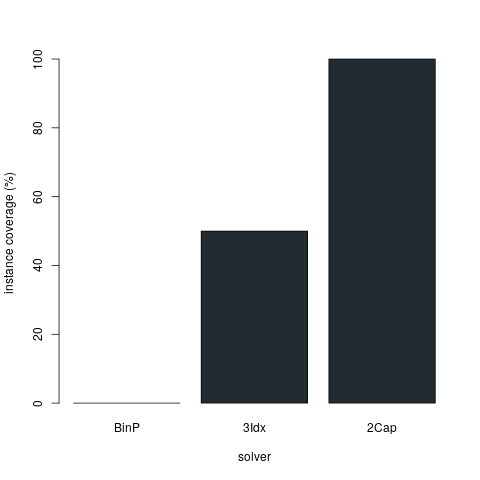
\includegraphics[width=0.3\textwidth]{images/solver_instance_coverage_b=2_s_1s.png}
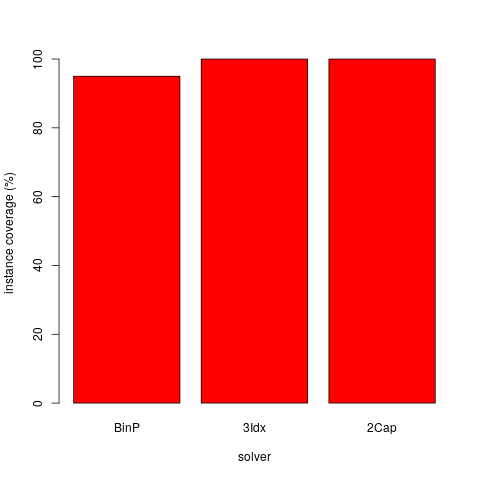
\includegraphics[width=0.3\textwidth]{images/solver_instance_coverage_b=2_s_3s.png}
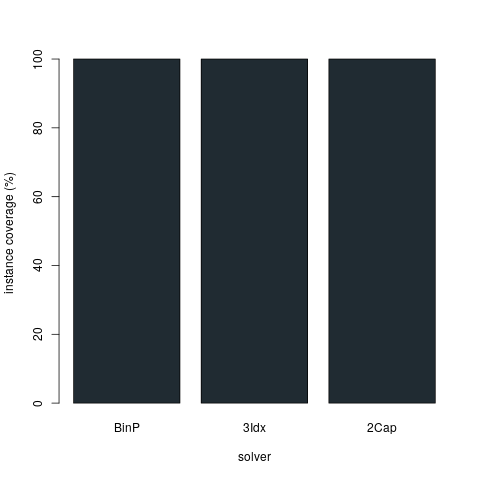
\includegraphics[width=0.3\textwidth]{images/solver_instance_coverage_b=2_s_5s.png}
\caption*{\textsc{Zeitlimit 1s} $\quad\quad\quad\quad$ \textsc{Zeitlimit 3s} $\quad\quad\quad\quad$ \textsc{Zeitlimit 5s}}
% \end{figure}
% \begin{figure}[H]
\begin{subfigure}[b]{0.3\textwidth}
\centering
\resizebox{\textwidth}{!}{
\begin{tabular}{ | l | l | l |}
    \hline
     & \textbf{BinP} & \textbf{3Idx} \\ \hline
    \textbf{Optimal} & $ \textcolor{red}{0 \%}$ & $ \textcolor{mygreen}{35 \%}$ \\ \hline
    \textbf{Laufzeit} & $\textcolor{red}{---}$ & \O $\thinspace \textcolor{mygreen}{0.9 s}$ \\ \hline
    \textbf{Abweichung} & $\textcolor{red}{---}$ & \O $\thinspace \textcolor{mygreen}{2.0 \%}$ \\ \hline
\end{tabular}}
\end{subfigure}
% $\quad\quad\quad\quad$
\begin{subfigure}[b]{0.3\textwidth}
\centering
\resizebox{\textwidth}{!}{
\begin{tabular}{ | l | l | l |}
    \hline
     & \textbf{BinP} & \textbf{3Idx} \\ \hline
    \textbf{Optimal} & $ \textcolor{red}{10 \%}$ & $ \textcolor{mygreen}{100 \%}$ \\ \hline
    \textbf{Laufzeit} & \O $\thinspace \textcolor{red}{3.0 s}$ & \O $\thinspace \textcolor{mygreen}{1.1 s}$ \\ \hline
    \textbf{Abweichung} & \O $\thinspace \textcolor{red}{4.7 \%}$ & \O $\thinspace \textcolor{mygreen}{0.0 \%}$ \\ \hline
\end{tabular}}
\end{subfigure}
% \end{figure}
% \begin{figure}[H]
\begin{subfigure}[b]{0.3\textwidth}
\centering
\resizebox{\textwidth}{!}{
\begin{tabular}{ | l | l | l |}
    \hline
     & \textbf{BinP} & \textbf{3Idx} \\ \hline
    \textbf{Optimal} & $ \textcolor{red}{90 \%}$ & $ \textcolor{mygreen}{100 \%}$ \\ \hline
    \textbf{Laufzeit} & \O $\thinspace \textcolor{red}{3.9 s}$ & \O $\thinspace \textcolor{mygreen}{1.1 s}$ \\ \hline
    \textbf{Abweichung} & \O $\thinspace \textcolor{red}{0.4 \%}$ & \O $\thinspace \textcolor{mygreen}{0.0 \%}$ \\ \hline
\end{tabular}}
\end{subfigure}
\end{figure}
\centering
\textbf{2Cap-Heuristik}\linebreak
\centering
Abweichung vom Optimum: \O $\thinspace \boldsymbol{2.0 \%}$\linebreak
\centering
Laufzeit: \O $\thinspace \boldsymbol{0.02 s}$

\end{frame}

\begin{frame}
\frametitle{Vergleich der $b = 2$ Solver (m)}

\begin{figure}
\centering
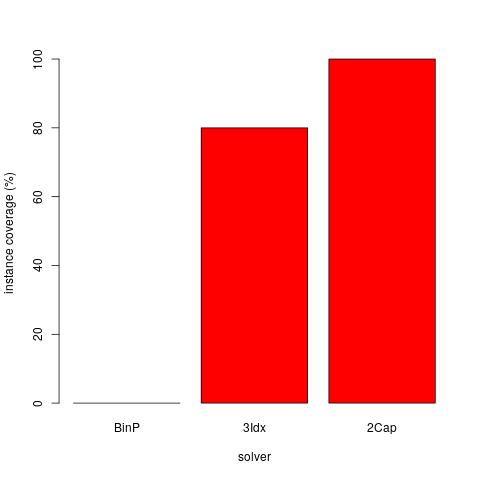
\includegraphics[width=0.3\textwidth]{images/solver_instance_coverage_b=2_m_60s.png}
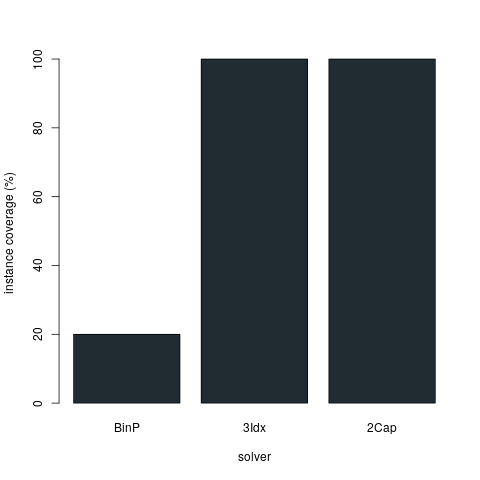
\includegraphics[width=0.3\textwidth]{images/solver_instance_coverage_b=2_m_600s.png}
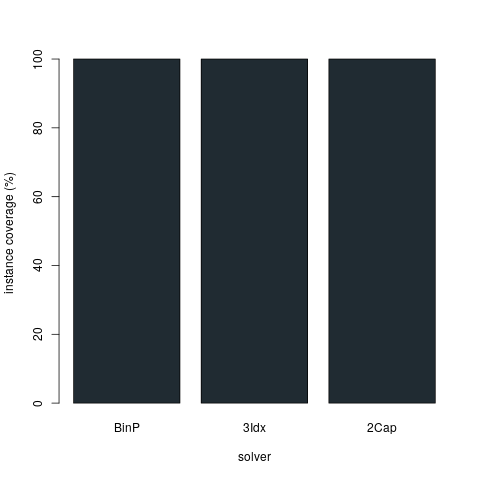
\includegraphics[width=0.3\textwidth]{images/solver_instance_coverage_b=2_m_1200s.png}
\caption*{\textsc{Zeitlimit 1min} $\quad\quad\quad$ \textsc{Zeitlimit 10min} $\quad\quad\quad$ \textsc{Zeitlimit 20min}}
% \end{figure}
% \begin{figure}[H]
% $\quad\quad\quad\quad$
\begin{subfigure}[b]{0.3\textwidth}
\centering
\resizebox{\textwidth}{!}{
\begin{tabular}{ | l | l | l |}
    \hline
     & \textbf{BinP} & \textbf{3Idx} \\ \hline
    \textbf{Optimal} & $ \textcolor{red}{0 \%}$ & $ \textcolor{mygreen}{50 \%}$ \\ \hline
    \textbf{Laufzeit} & $\textcolor{red}{---}$ & \O $\thinspace \textcolor{mygreen}{55.4 s}$ \\ \hline
    \textbf{Abweichung} & $\textcolor{red}{---}$ & \O $\thinspace \textcolor{mygreen}{0.8 \%}$ \\ \hline
\end{tabular}}
\end{subfigure}
\begin{subfigure}[b]{0.3\textwidth}
\centering
\resizebox{\textwidth}{!}{
\begin{tabular}{ | l | l | l |}
    \hline
     & \textbf{BinP} & \textbf{3Idx} \\ \hline
    \textbf{Optimal} & $ \textcolor{red}{10 \%}$ & $ \textcolor{mygreen}{100 \%}$ \\ \hline
    \textbf{Laufzeit} & \O $\thinspace \textcolor{red}{581.6 s}$ & \O $\thinspace \textcolor{mygreen}{73.7 s}$ \\ \hline
    \textbf{Abweichung} & \O $\thinspace \textcolor{red}{0.6 \%}$ & \O $\thinspace \textcolor{mygreen}{0.0 \%}$ \\ \hline
\end{tabular}}
\end{subfigure}
% \end{figure}
% \begin{figure}[H]
\begin{subfigure}[b]{0.3\textwidth}
\centering
\resizebox{\textwidth}{!}{
\begin{tabular}{ | l | l | l |}
    \hline
     & \textbf{BinP} & \textbf{3Idx} \\ \hline
    \textbf{Optimal} & $ 100 \%$ & $ 100 \%$ \\ \hline
    \textbf{Laufzeit} & \O $\thinspace 869.6 s$ & \O $\thinspace \textcolor{mygreen}{107.8 s}$ \\ \hline
    \textbf{Abweichung} & \O $\thinspace 0.0 \%$ & \O $\thinspace 0.0 \%$ \\ \hline
\end{tabular}}
\end{subfigure}
\end{figure}
\centering
\textbf{2Cap-Heuristik}\linebreak
\centering
Abweichung vom Optimum: \O $\thinspace \boldsymbol{0.8 \%}$\linebreak
\centering
Laufzeit: \O $\thinspace \boldsymbol{0.1 s}$

\end{frame}

\begin{frame}
\frametitle{Vergleich der $b = 2$ Solver (l)}

\begin{figure}
\centering
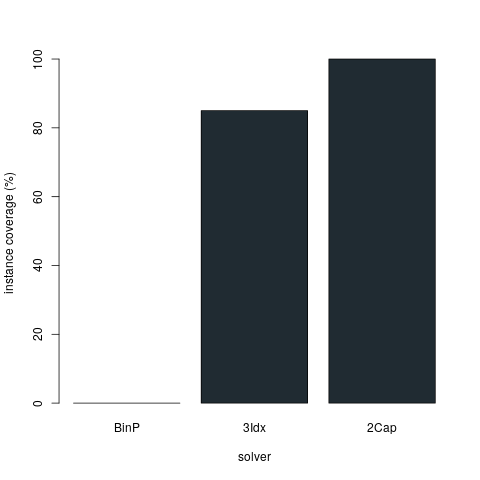
\includegraphics[width=0.3\textwidth]{images/solver_instance_coverage_b=2_l_1800s.png}

\includegraphics[width=0.3\textwidth]{images/na.png}

\includegraphics[width=0.3\textwidth]{images/na.png}
\caption*{\textsc{Zeitlimit 30min} $\quad\quad\quad$ \textsc{Zeitlimit 45min} $\quad\quad\quad$ \textsc{Zeitlimit 60min}}
% \end{figure}
% \begin{figure}[H]
\begin{subfigure}[b]{0.3\textwidth}
\centering
\resizebox{\textwidth}{!}{
\begin{tabular}{ | l | l | l |}
    \hline
     & \textbf{BinP} & \textbf{3Idx} \\ \hline
    \textbf{Optimal} & $  \%$ & $  \%$ \\ \hline
    \textbf{Laufzeit} & $---$ & \O $\thinspace 977.2 s$ \\ \hline
    \textbf{Abweichung} & \O $\thinspace  \%$ & \O $\thinspace  \%$ \\ \hline
\end{tabular}}
\end{subfigure}
% $\quad\quad\quad\quad$
\begin{subfigure}[b]{0.3\textwidth}
\centering
\resizebox{\textwidth}{!}{
\begin{tabular}{ | l | l | l |}
    \hline
     & \textbf{BinP} & \textbf{3Idx} \\ \hline
    \textbf{Optimal} & $  \%$ & $ \%$ \\ \hline
    \textbf{Laufzeit} & \O $\thinspace  s$ & \O $\thinspace  s$ \\ \hline
    \textbf{Abweichung} & \O $\thinspace \%$ & \O $\thinspace \%$ \\ \hline
\end{tabular}}
\end{subfigure}
% \end{figure}
% \begin{figure}[H]
\begin{subfigure}[b]{0.3\textwidth}
\centering
\resizebox{\textwidth}{!}{
\begin{tabular}{ | l | l | l |}
    \hline
     & \textbf{BinP} & \textbf{3Idx} \\ \hline
    \textbf{Optimal} & $ \%$ & $  \%$ \\ \hline
    \textbf{Laufzeit} & \O $\thinspace  s$ & \O $\thinspace s$ \\ \hline
    \textbf{Abweichung} & \O $\thinspace  \%$ & \O $\thinspace  \%$ \\ \hline
\end{tabular}}
\end{subfigure}
\end{figure}
\centering
\textbf{2Cap-Heuristik}\linebreak
\centering
Abweichung vom Optimum: \O $\thinspace \boldsymbol{ \%}$\linebreak
\centering
Laufzeit: \O $\thinspace \boldsymbol{0.7 s}$

\end{frame}

\begin{frame}
\frametitle{Konstruktive Heuristik ($b = 3$)}

\begin{itemize}
  \item Item-Paare bilden (\textsc{\textbf{MCM}(items)})
  \item Item-Tripel bilden (\textsc{\textbf{MCM}(pairs, unmatchedItems)})
  \item Verbleibende Item-Paare zu Tripeln mergen
  \item Item-Paare bilden (\textsc{\textbf{MCM}(remainingItems)})
  \item Verbleibende Items als \textquote{unmatched} betrachten
  \item Bipartiten Graph generieren:
  \begin{enumerate}
    \item Items (Item-Tripel, Item-Paare, Unmatched-Items)
    \item Stacks
  \end{enumerate}
  \item \textsc{\textbf{MWPM}} berechnen, Kanten als Stackzuweisungen interpretieren
  \item Ggf. Reihenfolge der Items innerhalb der Stacks anpassen
\end{itemize}
\end{frame}

\begin{frame}
\frametitle{Beispiel $b=3$}
$\boldsymbol{I} := \{0, 1, 2, 3, 4, 5, 6, 7, 8, 9\} \quad\quad\quad \boldsymbol{b} := 3 \quad\quad\quad \boldsymbol{m} := 4$
\begin{figure}[H]
\centering
\begin{tikzpicture}[scale=0.7, transform shape, node distance=2cm]
        \node[state] (A) {$\boldsymbol{\textcolor{mygreen}{0, 2}}$};
        \node[state] (B) [right of=A] {$\boldsymbol{\textcolor{mygreen}{1, 9}}$};
        \node[state] (C) [right of=B] {$\boldsymbol{\textcolor{mygreen}{3, 4}}$};
        \node[state] (D) [right of=C] {$\boldsymbol{\textcolor{mygreen}{5, 6}}$};
        \node[state] (E) [right of=D] {$\boldsymbol{\textcolor{red}{7}}$};
        \node[state] (F) [right of=E] {$\boldsymbol{\textcolor{red}{8}}$};
        \path;
  \end{tikzpicture}
  \caption*{\textsc{Item-Paare und Unmatched-Items}}
% \end{figure}
% \begin{figure}[H]
\centering
\begin{tikzpicture}[scale=0.7, transform shape, node distance=2cm]
        \node[state] (A) {$\boldsymbol{\textcolor{red}{0, 2}}$};
        \node[state] (B) [right of=A] {$\boldsymbol{\textcolor{red}{1, 9}}$};
        \node[state] (C) [right of=B] {$\boldsymbol{\textcolor{mygreen}{3, 4}}$};
        \node[state] (D) [below of =B] {$\boldsymbol{\textcolor{red}{5, 6}}$};
        \node[state] (E) [below of=A] {$\boldsymbol{\textcolor{mygreen}{7}}$};
        \node[state] (F) [below of=C] {$\boldsymbol{\textcolor{red}{8}}$};
        \path
          (E) edge [mygreen] node {} (C)
          (E) edge node {} (D);
  \end{tikzpicture}
  \caption*{\textsc{MCM aus Item-Paaren und Unmatched-Items}}
% \end{figure}
% \begin{figure}[H]
\centering
\begin{tikzpicture}[scale=0.7, transform shape, node distance=2cm]
        \node[state] (A) {$\boldsymbol{3, 4, 7}$};
        \node[state] (B) [right of=A] {$\boldsymbol{0, 2}$};
        \node[state] (C) [right of=B] {$\boldsymbol{1, 9}$};
        \node[state] (D) [right of=C] {$\boldsymbol{5, 6}$};
        \node[state] (E) [right of=D] {$\boldsymbol{8}$};
        \path;
  \end{tikzpicture}
  \caption*{\textsc{Item-Tripel, Item-Paare und Unmatched-Items}}
\end{figure}
\end{frame}

\begin{frame}
\frametitle{Beispiel $b=3$}

\begin{figure}[H]
\begin{subfigure}[b]{0.4\textwidth}
\centering
\begin{tikzpicture}[scale=0.45, transform shape, node distance=2cm]
        \node[state] (A) {$\boldsymbol{0, 2}$};
        \node[state] (B) [right of=A] {$\boldsymbol{1, 9}$};
        \node[state] (C) [right of=B] {$\boldsymbol{5, 6}$};
        \path;
  \end{tikzpicture}
  \caption*{\textsc{Item-Paare}}
\end{subfigure}
\hfill
\begin{subfigure}[b]{0.4\textwidth}
\centering
\begin{tikzpicture}[scale=0.45, transform shape, node distance=2cm]
        \node[state] (A) {$\boldsymbol{0, 5, 6}$};
        \node[state] (B) [right of=A] {$\boldsymbol{2, 1, 9}$};
        \path;
  \end{tikzpicture}
  \caption*{\textsc{Merge-Ergebnis}}
\end{subfigure}
% \end{figure}
\newline\newline
% \begin{figure}[H]
\begin{subfigure}[b]{0.4\textwidth}
\centering
\begin{tikzpicture}[scale=0.5, transform shape, node distance=2cm]
        \node[state] (A) {$\boldsymbol{3, 4, 7}$};
        \node[state] (B) [below of=A] {$\boldsymbol{0, 5, 6}$};
        \node[state] (C) [below of=B] {$\boldsymbol{2, 1, 9}$};
        \node[state] (D) [below of=C] {$\boldsymbol{8}$};

        \node[state] (E) [right = 4cm of A] {$\boldsymbol{S_1}$};
        \node[state] (F) [below of=E] {$\boldsymbol{S_2}$};
        \node[state] (G) [below of=F] {$\boldsymbol{S_3}$};
        \node[state] (H) [below of=G] {$\boldsymbol{S_4}$};

        \path
          (A) edge node {} (E)
          (A) edge node {} (F)
          (A) edge node {} (G)
          (A) edge node {} (H)

          (B) edge node {} (E)
          (B) edge node {} (F)
          (B) edge node {} (G)
          (B) edge node {} (H)

          (C) edge node {} (E)
          (C) edge node {} (F)
          (C) edge node {} (G)
          (C) edge node {} (H)

          (D) edge node {} (E)
          (D) edge node {} (F)
          (D) edge node {} (G)
          (D) edge node {} (H);
  \end{tikzpicture}
  \caption*{\textsc{Vollständig Bipartit}}
\end{subfigure}
\hfill
\begin{subfigure}[b]{0.4\textwidth}
\centering
\begin{tikzpicture}[scale=0.5, transform shape, node distance=2cm]
        \node[state] (A) {$\boldsymbol{3, 4, 7}$};
        \node[state] (B) [below of=A] {$\boldsymbol{0, 5, 6}$};
        \node[state] (C) [below of=B] {$\boldsymbol{2, 1, 9}$};
        \node[state] (D) [below of=C] {$\boldsymbol{8}$};

        \node[state] (E) [right = 4cm of A] {$\boldsymbol{S_1}$};
        \node[state] (F) [below of=E] {$\boldsymbol{S_2}$};
        \node[state] (G) [below of=F] {$\boldsymbol{S_3}$};
        \node[state] (H) [below of=G] {$\boldsymbol{S_4}$};

        \path
          (A) edge node {} (H)
          (B) edge node {} (F)
          (C) edge node {} (G)
          (D) edge node {} (E);
  \end{tikzpicture}
  \caption*{\textsc{MWPM}}
\end{subfigure}
% \end{figure}
\newline
% \begin{figure}[H]
  \centering
  \resizebox{0.3\textwidth}{!}{
    \begin{tabular}{c|c|c|c|c|}
    \cline{2-5}
    $\boldsymbol{L_3}$ & $$ & $6$ & $9$ & $7$ \\ \cline{2-5}
    $\boldsymbol{L_2}$ & $$ & $5$ & $1$ & $4$ \\ \cline{2-5}
    $\boldsymbol{L_1}$ & $8$ & $0$ & $2$ & $3$ \\ \cline{2-5}
    \multicolumn{1}{c}{} & \multicolumn{1}{c}{$\boldsymbol{S_1}$} & \multicolumn{1}{c}{$\boldsymbol{S_2}$}
    & \multicolumn{1}{c}{$\boldsymbol{S_3}$} & \multicolumn{1}{c}{$\boldsymbol{S_4}$} \\
    \end{tabular}}
    \caption*{\textsc{Zulässige Zuweisungen (ggf. Item-Reihenfolge korrigieren)}}
\end{figure}

\end{frame}

\begin{frame}
\frametitle{Vergleich der $b = 3$ Solver (s)}

\begin{figure}
\centering
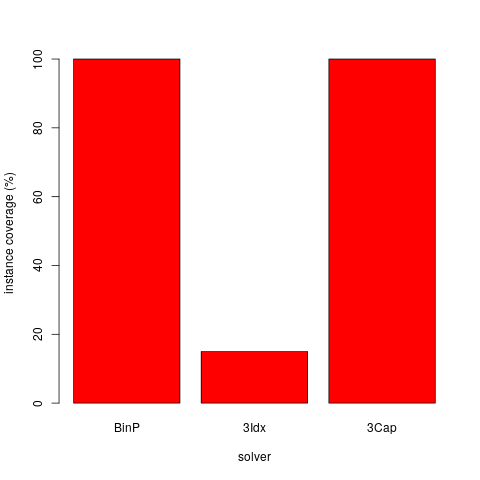
\includegraphics[width=0.3\textwidth]{images/solver_instance_coverage_b=3_small_3s.png}
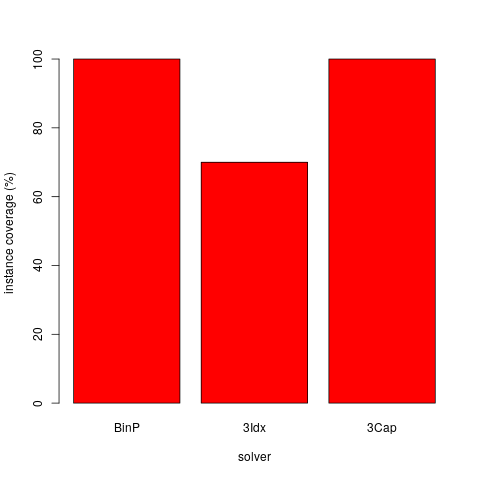
\includegraphics[width=0.3\textwidth]{images/solver_instance_coverage_b=3_small_5s.png}
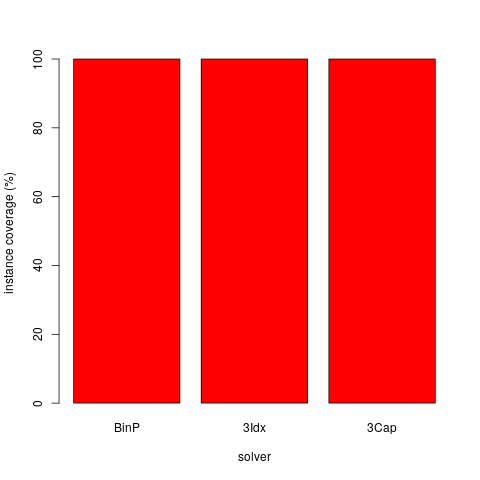
\includegraphics[width=0.3\textwidth]{images/solver_instance_coverage_b=3_small_10s.png}
\caption*{\textsc{Zeitlimit 3s} $\quad\quad\quad\quad$ \textsc{Zeitlimit 5s} $\quad\quad\quad\quad$ \textsc{Zeitlimit 10s}}
% \end{figure}
% \begin{figure}[H]
% $\quad\quad\quad\quad$
\begin{subfigure}[b]{0.3\textwidth}
\centering
\resizebox{\textwidth}{!}{
\begin{tabular}{ | l | l | l |}
    \hline
     & \textbf{BinP} & \textbf{3Idx} \\ \hline
    \textbf{Optimal} & $\textcolor{mygreen}{40 \%}$ & $\textcolor{red}{5 \%}$ \\ \hline
    \textbf{Laufzeit} & \O $\thinspace 2.9 s$ & \O $\thinspace 2.9 s$ \\ \hline
    \textbf{Abweichung} & \O $\thinspace \textcolor{mygreen}{1.7 \%}$ & \O $\thinspace \textcolor{red}{7.8 \%}$ \\ \hline
\end{tabular}}
\end{subfigure}
% \end{figure}
% \begin{figure}[H]
\begin{subfigure}[b]{0.3\textwidth}
\centering
\resizebox{\textwidth}{!}{
\begin{tabular}{ | l | l | l |}
    \hline
     & \textbf{BinP} & \textbf{3Idx} \\ \hline
    \textbf{Optimal} & $\textcolor{mygreen}{100 \%}$ & $\textcolor{red}{50 \%}$ \\ \hline
    \textbf{Laufzeit} & \O $\thinspace \textcolor{mygreen}{3.1 s}$ & \O $\thinspace \textcolor{red}{4.0 s}$ \\ \hline
    \textbf{Abweichung} & \O $\thinspace \textcolor{mygreen}{0.0 \%}$ & \O $\thinspace \textcolor{red}{1.2 \%}$ \\ \hline
\end{tabular}}
\end{subfigure}
\begin{subfigure}[b]{0.3\textwidth}
\centering
\resizebox{\textwidth}{!}{
\begin{tabular}{ | l | l | l |}
    \hline
     & \textbf{BinP} & \textbf{3Idx} \\ \hline
    \textbf{Optimal} & $ \textcolor{mygreen}{100 \%}$ & $ \textcolor{red}{85 \%}$ \\ \hline
    \textbf{Laufzeit} & \O $\thinspace \textcolor{mygreen}{3.1 s}$ & \O $\thinspace \textcolor{red}{5.6 s}$ \\ \hline
    \textbf{Abweichung} & \O $\thinspace \textcolor{mygreen}{0.0 \%}$ & \O $\thinspace \textcolor{red}{0.5 \%}$ \\ \hline
\end{tabular}}
\end{subfigure}
\end{figure}
\centering
\textbf{3Cap-Heuristik}\linebreak
\centering
Abweichung vom Optimum: \O $\thinspace \boldsymbol{2.65 \%}$\linebreak
\centering
Laufzeit: \O $\thinspace \boldsymbol{0.01s}$

\end{frame}

\begin{frame}
\frametitle{Vergleich der $b = 3$ Solver (m)}

\begin{figure}
\centering
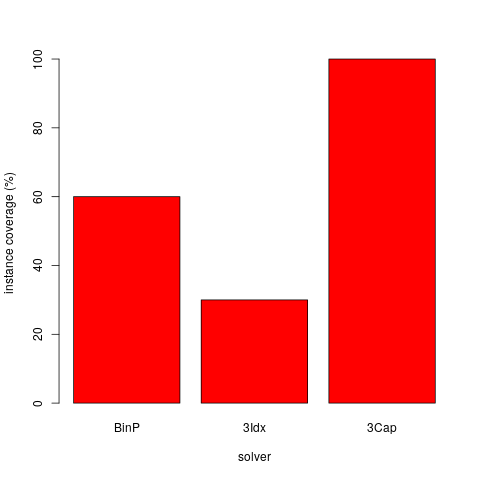
\includegraphics[width=0.3\textwidth]{images/solver_instance_coverage_b=3_medium_600s.png}
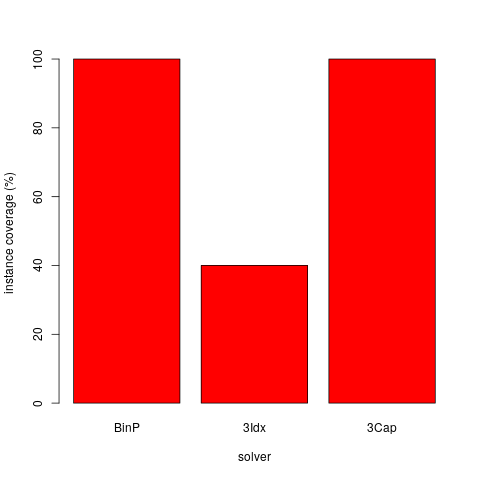
\includegraphics[width=0.3\textwidth]{images/solver_instance_coverage_b=3_medium_1200s.png}
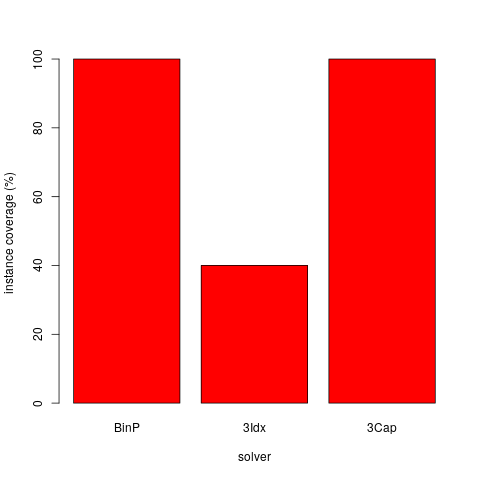
\includegraphics[width=0.3\textwidth]{images/solver_instance_coverage_b=3_medium_1800s.png}
\caption*{\textsc{Zeitlimit 10min} $\quad\quad\quad$ \textsc{Zeitlimit 20min} $\quad\quad\quad$ \textsc{Zeitlimit 30min}}
% \end{figure}
% \begin{figure}[H]
\begin{subfigure}[b]{0.3\textwidth}
\centering
\resizebox{\textwidth}{!}{
\begin{tabular}{ | l | l | l |}
    \hline
     & \textbf{BinP} & \textbf{3Idx} \\ \hline
    \textbf{Optimal} & $ \textcolor{mygreen}{20 \%}$ & $ \textcolor{red}{10 \%}$ \\ \hline
    \textbf{Laufzeit} & \O $\thinspace \textcolor{red}{583.7 s}$ & \O $\thinspace \textcolor{mygreen}{554.3 s}$ \\ \hline
    \textbf{Abweichung} & \O $\thinspace \textcolor{red}{0.2 \%}$ & \O $\thinspace \textcolor{mygreen}{0.01 \%}$ \\ \hline
\end{tabular}}
\end{subfigure}
% $\quad\quad\quad\quad$
\begin{subfigure}[b]{0.3\textwidth}
\centering
\resizebox{\textwidth}{!}{
\begin{tabular}{ | l | l | l |}
    \hline
     & \textbf{BinP} & \textbf{3Idx} \\ \hline
    \textbf{Optimal} & $ \textcolor{mygreen}{100 \%}$ & $ \textcolor{red}{30 \%}$ \\ \hline
    \textbf{Laufzeit} & \O $\thinspace \textcolor{mygreen}{791.4 s}$ & \O $\thinspace \textcolor{red}{795.4 s}$ \\ \hline
    \textbf{Abweichung} & \O $\thinspace 0.0 \%$ & \O $\thinspace 0.0 \%$ \\ \hline
\end{tabular}}
\end{subfigure}
% \end{figure}
% \begin{figure}[H]
\begin{subfigure}[b]{0.3\textwidth}
\centering
\resizebox{\textwidth}{!}{
\begin{tabular}{ | l | l | l |}
    \hline
     & \textbf{BinP} & \textbf{3Idx} \\ \hline
    \textbf{Optimal} & $ \textcolor{mygreen}{100 \%}$ & $ \textcolor{red}{35 \%}$ \\ \hline
    \textbf{Laufzeit} & \O $\thinspace \textcolor{mygreen}{766.4 s}$ & \O $\thinspace \textcolor{red}{874.0 s}$ \\ \hline
    \textbf{Abweichung} & \O $\thinspace 0.0 \%$ & \O $\thinspace 0.0 \%$ \\ \hline
\end{tabular}}
\end{subfigure}
\end{figure}
\centering
\textbf{3Cap-Heuristik}\linebreak
\centering
Abweichung vom Optimum: \O $\thinspace \boldsymbol{1.02 \%}$\linebreak
\centering
Laufzeit: \O $\thinspace \boldsymbol{0.2 s}$

\end{frame}

\begin{frame}
\frametitle{Vergleich der $b = 3$ Solver (l)}

\begin{figure}
\centering
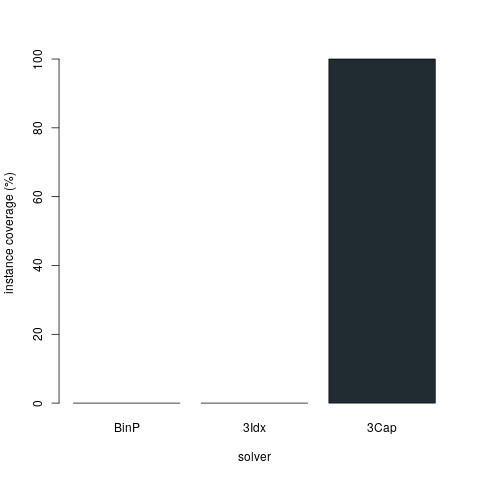
\includegraphics[width=0.3\textwidth]{images/solver_instance_coverage_b=3_l_1800s.png}

\includegraphics[width=0.3\textwidth]{images/na.png}

\includegraphics[width=0.3\textwidth]{images/na.png}
\caption*{\textsc{Zeitlimit 30min} $\quad\quad\quad$ \textsc{Zeitlimit 45min} $\quad\quad\quad$ \textsc{Zeitlimit 60min}}
% \end{figure}
% \begin{figure}[H]
\begin{subfigure}[b]{0.3\textwidth}
\centering
\resizebox{\textwidth}{!}{
\begin{tabular}{ | l | l | l |}
    \hline
     & \textbf{BinP} & \textbf{3Idx} \\ \hline
    \textbf{Optimal} & $ \textcolor{red}{0 \%}$ & $ \textcolor{red}{0 \%}$ \\ \hline
    \textbf{Laufzeit} & $\textcolor{red}{---}$ & $\textcolor{red}{---}$ \\ \hline
    \textbf{Abweichung} & $\textcolor{red}{---}$ & $\textcolor{red}{---}$ \\ \hline
\end{tabular}}
\end{subfigure}
% $\quad\quad\quad\quad$
\begin{subfigure}[b]{0.3\textwidth}
\centering
\resizebox{\textwidth}{!}{
\begin{tabular}{ | l | l | l |}
    \hline
     & \textbf{BinP} & \textbf{3Idx} \\ \hline
    \textbf{Optimal} & $  \%$ & $ \%$ \\ \hline
    \textbf{Laufzeit} & \O $\thinspace  s$ & \O $\thinspace  s$ \\ \hline
    \textbf{Abweichung} & \O $\thinspace \%$ & \O $\thinspace \%$ \\ \hline
\end{tabular}}
\end{subfigure}
% \end{figure}
% \begin{figure}[H]
\begin{subfigure}[b]{0.3\textwidth}
\centering
\resizebox{\textwidth}{!}{
\begin{tabular}{ | l | l | l |}
    \hline
     & \textbf{BinP} & \textbf{3Idx} \\ \hline
    \textbf{Optimal} & $ \%$ & $  \%$ \\ \hline
    \textbf{Laufzeit} & \O $\thinspace  s$ & \O $\thinspace s$ \\ \hline
    \textbf{Abweichung} & \O $\thinspace  \%$ & \O $\thinspace  \%$ \\ \hline
\end{tabular}}
\end{subfigure}
\end{figure}
\centering
\textbf{3Cap-Heuristik}\linebreak
\centering
Abweichung vom Optimum: \O $\thinspace \boldsymbol{ \%}$\linebreak
\centering
Laufzeit: \O $\thinspace \boldsymbol{1.0 s}$

\end{frame}

%------------------------------------------------
\section{Ausblick}
%------------------------------------------------
% \subsection*{}

\begin{frame}
\frametitle{Ausblick}
\begin{itemize}
  \item Konstruktive Heuristik für $\boldsymbol{b = 4}$ entwickeln
  \item Verbesserungsverfahren implementieren
  \item Realistischere Test-Instanzen basierend auf \textbf{Briskorn (2018)}
  \item Einfluss von $\boldsymbol{m}$ auf die Schwierigkeit des Problems untersuchen ($+20\%$, +30\%, ...)
  \item Evaluation
\end{itemize}
\end{frame}

% %------------------------------------------------

% \begin{frame}[c,plain]
% \centering
% \Huge{\textcolor{quat}{Danke für eure Aufmerksamkeit!\\[1cm] Fragen?}}
% \end{frame}

% %------------------------------------------------

\end{document}
